\begin{figure}[tbp]
\begin{center}
\includegraphics[width=0.4\textwidth]{compare_bias_rsdsub_z1z2.eps}
\end{center}
\vspace{-0.7cm}
\caption{The bias $b=P_{\delta_\mathrm{nlRSD},\delta}/P_{\delta}$ 
of redshift space distorted(RSD) field after linear RSD substraction.
Dark lines indicate the $k_c$ cutoff---modes above them are assumed to be lost in noise.}
\label{fig:bias}
\end{figure}
The redshift space distortion(RSD) refers to the misjudgement on comoving distance 
results from peculiar velocity of objects. 
In this section we add the RSD effect to our original fields and study its influence on our reconstruction. 

%$\chi^{RSD}=\chi+\frac{v_z}{H}$, 
%where $\chi$ is the radial distance, $v_z$ is the parallel peculiar velocity.
Linearly, RSD induces an additional contraction in $z$ direction 
$\delta^{RSD}(\bm{k})=(1+f\mu^2)\delta(\bm{k})$. 
where $\mu=\frac{k_\parallel}{k}$. 
We can easily filter it by dividing the observed density contrast with $1+f\mu^2$. 
However, for low redshift, non-linear effect may also play a role.
Substracting the linear RSD, we present the bias between the remaining RSD field 
and field in real space 
$b=P_{\delta_\mathrm{nlRSD},\delta}/P_{\delta}$  
in Fig.\ref{fig:bias}. 
Dark lines indicate the $k_c$ cutoff---modes above them are assumed to be lost in noise.

For z=2, the modes we can obtain in real observations are generally 
within linear RSD regions. 
However, for z=1, there are sufficient non-linear effects below $k_c=0.5$ h/Mpc, which cannot be filtered out directly in this way.  

A better yet troublesome way to substract RSD is 
first performing tidal reconstruction on RSD field, 
then using recovered large scale modes to calculate linear velocity field 
and substracting the velocity in RSD field.  
Since nonlinearity in velocity field is less severe than in density field, 
this method should work better than direct substraction on density field, 
especially if we do it iterately.

Besides this, there is a less optimal yet much more convenient way to deal 
with RSD---to leave it still. 
The linear contraction still dominates the RSD, 
nd its rule is the large $k_z$ is, the stronger the contraction. 
The result is presented in Fig.\ref{fig:r}. 

Much to our surprise, the cross correlation is even improved by 0.1. 
This is possibly because both RSD and foregrounds are in z direction. 
The contraction induced by RSD assigns more weigh to large $k_z$ modes, 
and these are the most clean signals survived from foregrounds.  
Moreover, RSD assigns more weigh to shear estimators related to covariance in z directions, 
and this is where best tidal recovered modes come from.  
Hence, the field with RSD accidentally give us better results on cross correlation.

This is not the only advantage RSD brings. 
Actually the inhancement in large $k_z$ will increase the S/N at that level, 
raise the cut off scale $k_c$ and ultimately improve the reconstruction results. 
In all, redshift space distortion seems to be a blessing rather than problem in our case. 
